

\chapter{Design}
\label{ch:design}
The design of the project consists of three individual sections: The Emulator \ref{sec:emulator}, Visualisation \ref{sec:visualisation} and the Module System \ref{sec:module}, which later combine to produce the final application. The module system was not originally a section, but was considered later on and then designed to allow for RISC-V extensions to be included. The use of "extension" and "module" may be confused within this section. Modules and extensions should be identified as follows: "We create a \textbf{module} that encapsulates the logic of a RISC-V \textbf{extension}".

This approach was chosen to allow for a consistent flow of development, with the Emulator being core, thus allowing the visualisation system to know what to simulate. Hence, the emulator must be completed first, then the visualisation built separately, and then later being combined on top of the emulator. The module system can then be intertwined later once it is designed. 

Together these 3 sections encapsulate the entire project and its complete functionality. The inclusion of the Module system allows us to satisfy requirements \ref{req:md} and \ref{req:fp} to include the Multiply and Divide, and Single Precision Floating Point Module. With these 3 sections being created completely from scratch it provides the flexibility to independently design and create each. Then combining them later on when required, allowing for a detached design and implementation process.

\begin{figure}[h]
    \centering
    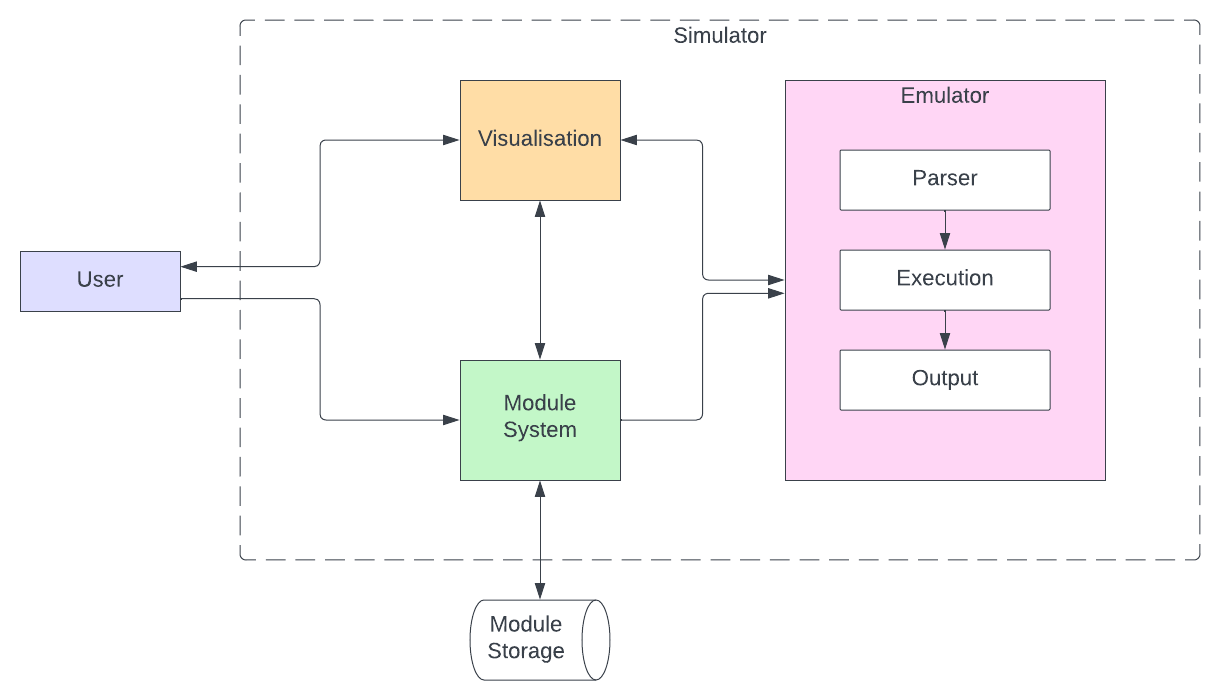
\includegraphics[width=0.95\linewidth]{dissertation/DATA/sys architecture.png}
    \caption{Overall System Architecture}
    \label{fig:sys_architecture}
\end{figure}

In the system architecture diagram in Figure \ref{fig:sys_architecture} we provide an outline of how the 3 sections integrate within the simulator. A user will directly interact with the visualisation layer, in turn the visualisation layer interacts directly with the emulator and module system to provide functionality. This approach was decided upon as the end user should never directly interact with the emulator as this avoids the simulation aspect. The user should also have limited access to the module system, being restricted to just enabling, disabling, loading and unloading modules as they require, without having to worry about the underlying effects on the rest of the visualisation and emulation systems.

Within the system architecture diagram "Module Storage" is denoted. This storage will exist on the users physical machine, storing  module Jars such that added functionality can persist over application restarts.

It is important to consider how a user may interact with the system in everyday use. The user sequence diagram in Figure \ref{fig:user_sequence} describes a typical user flow. The flow covers how a user may start by launching the application and entering a RISC-V program.

By hitting "Run" the code is either accepted via a successful parse or rejected and a error is returned to the user. This may repeat several times, until a successful parse occurs. When this happens the program is executed line per line with animations playing out sequentially. After the user may decide to manage their modules via the module popup. Enabling or disabling the listed modules, with a confirmation being shown after each change.

\begin{figure}[h]
    \centering
    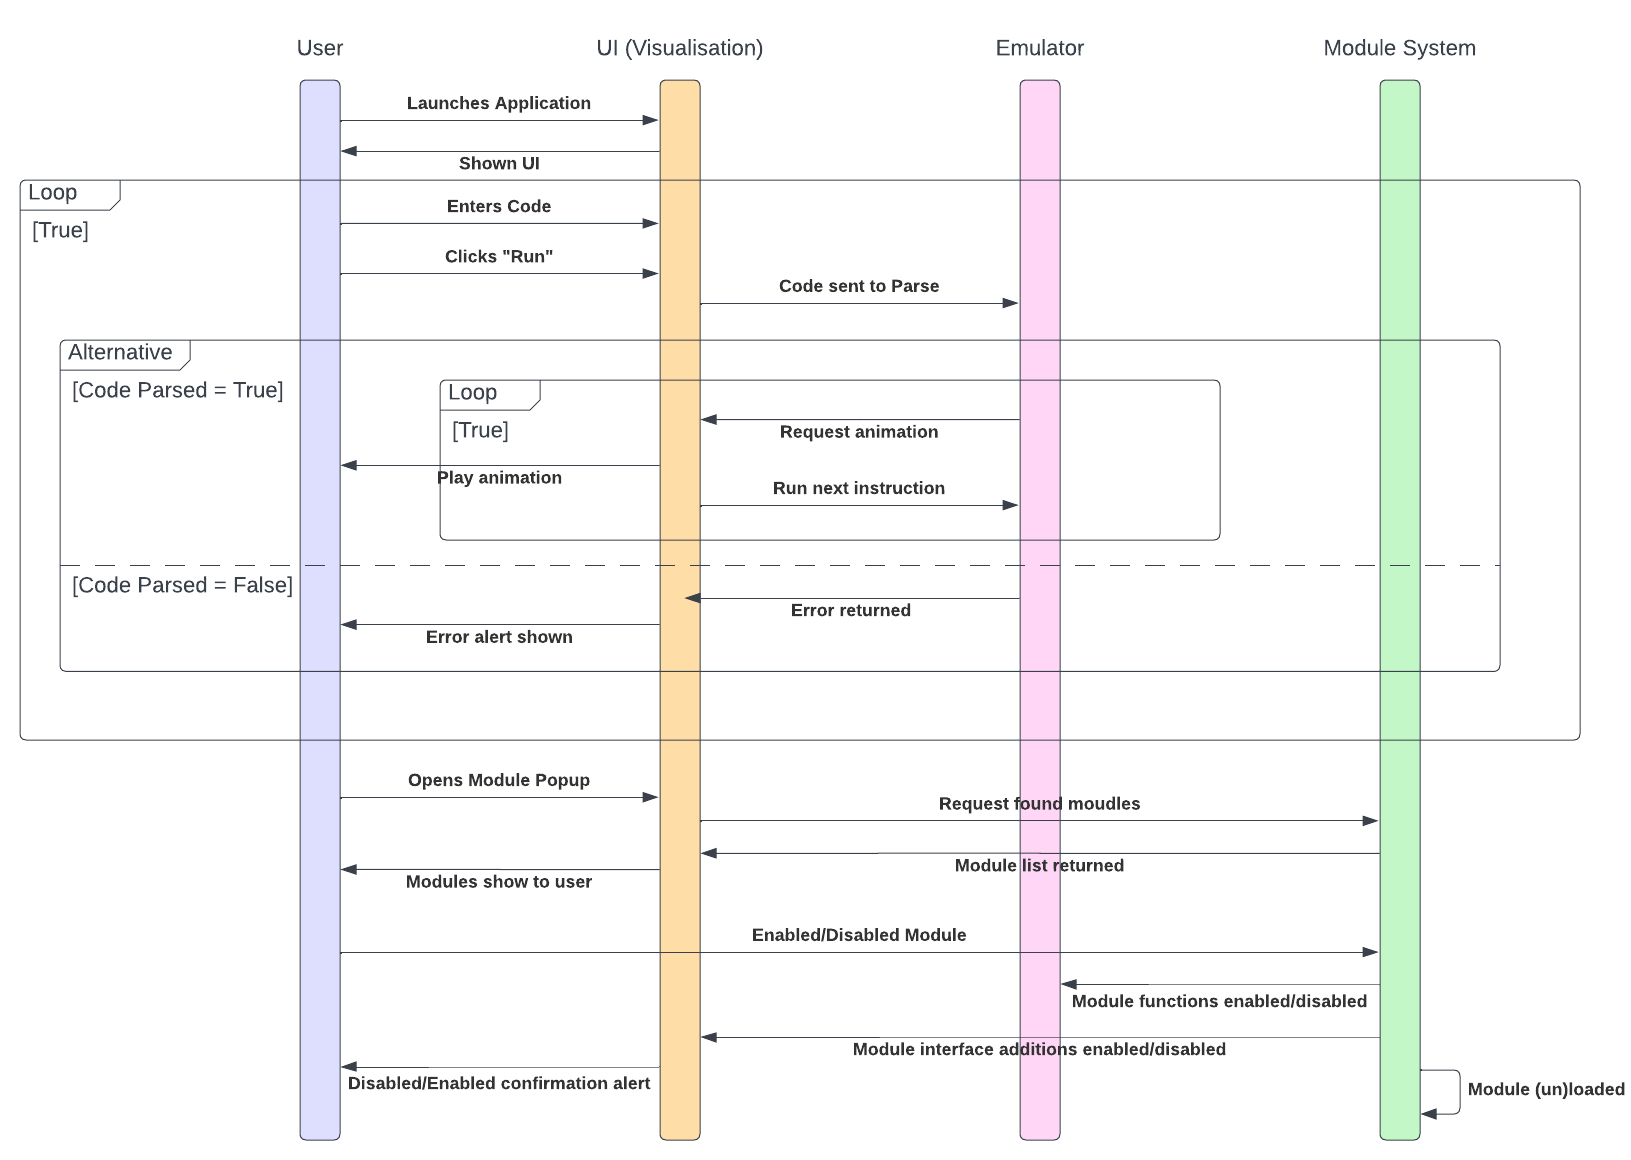
\includegraphics[width=0.95\linewidth]{dissertation/DATA/sequence diagram.png}
    \caption{Example user sequence diagram}
    \label{fig:user_sequence}
\end{figure}

\section{Emulator}\label{sec:emulator}
The emulator is designed to mock the RISC-V architecture closely, whilst also being simple and efficient. In the overall system architecture diagram in Figure \ref{fig:sys_architecture} the emulator is denoted as flowing between 3 high level ideas: "Parser", "Execution" and "Output". These are not rigid names, but allow us to comprise a high level overview of the entire emulator with each being discussed below:

\subsection{Parser}\label{sec:parser}
In order for any code to be emulated it must be parsed first. The design for the parser must be simple and efficient, providing suitable error feedback when required.

The parser is designed to consume the inputted user program line-by-line. Each line is expected to conform to a valid instruction with a set amount of operands. For example the following valid ADDI instruction will read register x1, add 3 to it and then write the result back to register x1:\\\\
\verb|ADDI x1, x1, 3|
\\\\
The parser should first identify the instruction name, and then identify the respective operands that the instruction should expect, including how many and of what type. This can be performed linearly by consuming each inputted operand and checking if it conforms to the expected type, whilst pre-checking there aren't more or less operands than expected. The parser will reject on any invalid operands or instructions, throwing an exception if so. If an instruction is valid, it should be completely consumed and converted into an intermediary instruction format (as described below) for use later.

\begin{figure}[H]
    \centering
    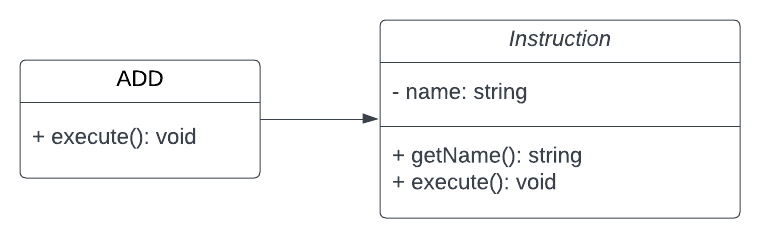
\includegraphics[width=0.95\linewidth]{dissertation/DATA/instr_abstract_uml.png}
    \caption{Basic UML diagram of the Abstract instruction class}
    \label{fig:instr_abstract_uml}
\end{figure}

Figure \ref{fig:instr_abstract_uml} presents this intermediary form. This abstract \texttt{Instruction} class will encapsulate each individual instructions logic, with every instruction extending and overriding the \verb|execute()| method. Figure \ref{fig:instr_abstract_uml} shows an example of an ADD instruction being implemented.

Each individual implementation should be stored centrally and referred to by name such that it may be called later for execution. The parsed operands should be stored separately such that each instruction may be reused with different operand combinations.


\subsection{Execution}
Execution encapsulates the internal design of the system including the Registers, Memory, and how they integrate. There needs to be a consideration first on how both will store a 32 bit binary value. This could simply be a string of 32$\times$1's and 0's or the base Java integer type.

However, the use of a custom \texttt{Binary} object \ref{fig:bin_regmem_uml} would seem more logical to provide consistency between the Register and Memory. This \texttt{Binary} object would contain simple functions to read and write as Binary, Denary and Hexadecimal.

The emulation requires a representation of the 32 base registers, with the ability to reference them by not only their name, but also their respective Application Binary Interface (ABI) name as well \cite{riscvinternational_2014_calling}(page 3). The ABI is an alternate name denoting specific usage or ideal placement of data. 

A list might work nicely here, allowing direct addressing from 0-31 for the base 31 registers, however if the user addressed via the ABI name we would have to linearly search every register to check its ABI name which is inefficient. Thus, a map suits the problem better, with the ability to directly map both the numerical name and ABI name to each register. Then each can be read and written via these names as seen in Figure \ref{fig:bin_regmem_uml}. Providing a O(1) lookup time as an additional benefit.

Unlike registers, memory needs to be addressable by its 4 byte aligned location, and thus we could opt for two methods of referencing:
\begin{enumerate}
    \item Use a list and take modulo 4 of the address to get the relative index in the list for each memory value.
    \item Use a map to store the location as a key, with the memory value as the value, avoiding extra computation to calculate locations.
\end{enumerate}
Both are valid options. However, option 2 provides the benefit of a O(1) lookup time, compared to O(n) for a list. And, seeing as the memory may become infinitely large with a complex emulation, option 2 is by far the better choice with the O(1) lookup time.

\begin{figure}[H]
    \centering
    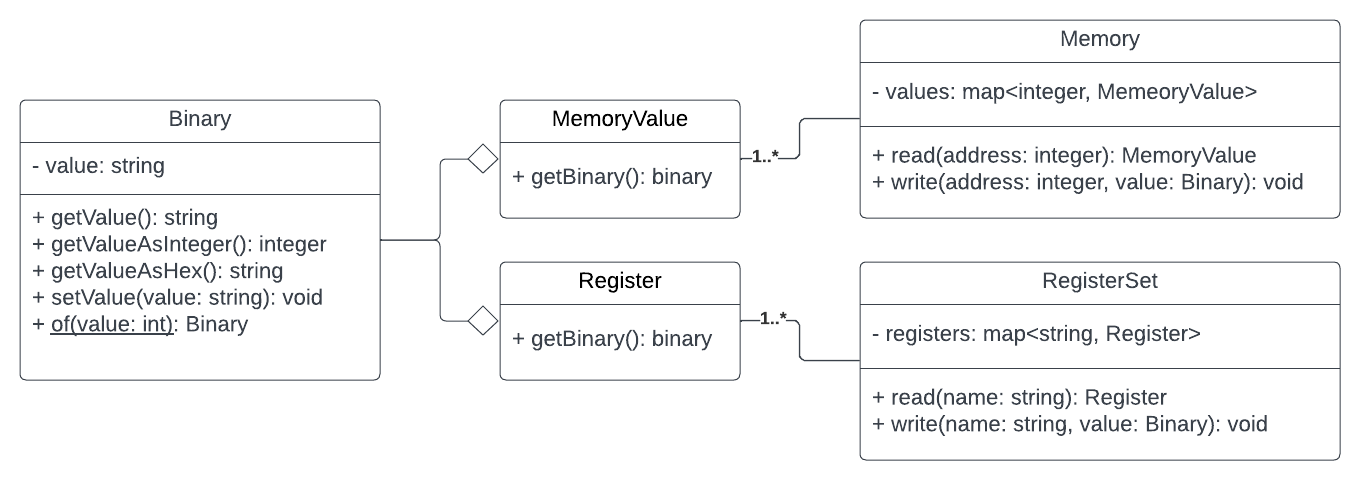
\includegraphics[width=\linewidth]{dissertation/DATA/bin_regmem_uml.png}
    \caption{Binary, Memory and Register UML Diagram}
    \label{fig:bin_regmem_uml}
\end{figure}

\subsection{Output}
Our output design simply comes in the form of the handshake between the emulator and the visualisation. The Emulator itself should only output the end result, parse errors and signals for animations to take place.

These should be simple to differentiate. Most likely with parse errors being raised that can be caught and passed to the visualisation to be displayed. Then, the end output can be printed to the terminal during development and also utilised for debugging. Finally, the animation signals can be preemptively stubbed in code, and later hooked into the visualisation system.

\section{Visualisation}\label{sec:visualisation}
The visualisation of the emulation is one of the larger parts of the project, with the overall simulation relying heavily on a well designed \ac{UI}. Thus, the design of the \ac{UI} has been heavily considered to ensure an appropriate interface is developed that presents the right amount of information without being too simple or complicated.

\begin{figure}[H]
    \centering
    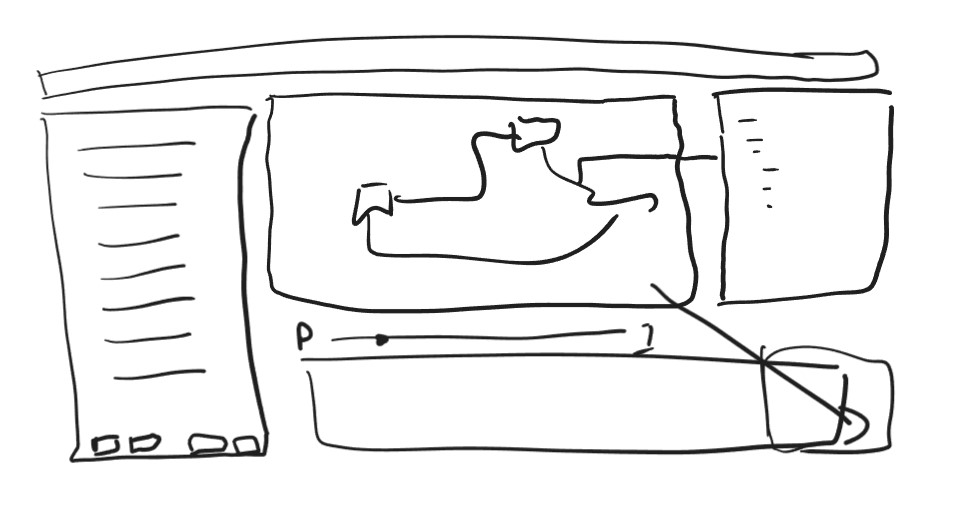
\includegraphics[width=\linewidth]{dissertation/DATA/early_design.jpg}
    \caption{Original hand drawn UI design}
    \label{fig:early_ui_design}
\end{figure}

Our first \ac{UI} design (Figure \ref{fig:early_ui_design}) was designed to be basic. Being loosely designed of LittleManComputer (Figure \ref{fig:lmc}) and Emulsiv (Figure \ref{fig:emulsiv}).

The design places the code editor on the left, the main visualisation area in the centre, registers on the right, memory along the bottom and a menu bar stretching the top. These positions were specifically chosen based on the constraint of element sizing:
\begin{itemize}
    \item The code editor requires a large vertical space to hold many lines of code. But a relatively short horizontal width, due to the average instruction being relatively short.
    \item The animation/visualisation area was given the most space as this is the main focus point of the application, and thus being dead centre is the most appropriate location within the \ac{UI}.
    \item Registers, much like the code editor require a small horizontal space to display their value. But 32 of them need to be on display at any given time, thus a large horizontal space allows for this with minimal scrolling on smaller screens.
    \item Memory also requires limited horizontal space however, unlike registers, it starts off empty for every execution, and may not be used in any given execution. Thus, designating it to the bottom of the screen to fill waste space is more appropriate. Should the memory fill up, the user may scroll through it to see all the values at any given time.
\end{itemize}

Other elements have also been positioned for their own respective reasons irrespective of size constraints:
\begin{itemize}
    \item The menu bar stretches along the top to conform with expected user patterns and expectations. With users commonly expecting it at the top of the application, placing it elsewhere would of been unintuitive.
    \item The Settings and Module sections are represented as popups displaying in the middle of the screen. This conforms with other applications, whilst grabbing attention to the popup without users having to search for it on screen. It also provides the option to be moved based on the users need, whilst hiding secondary content that is less important to the core system.
\end{itemize}

As-well as the overall \ac{UI} design, a intuitive layout needed to be created to visualise the internal data movement around the processor components (\ac{ALU}, \ac{CU}, \ac{IR}, \ac{ID}, Instruction Memory, Registers and Memory). The original design of this can be seen below in Figure \ref{fig:early_animation_design} with, Control Unit designs in Figure \ref{fig:early_cu_design}.

\begin{figure}[H]
    \centering
    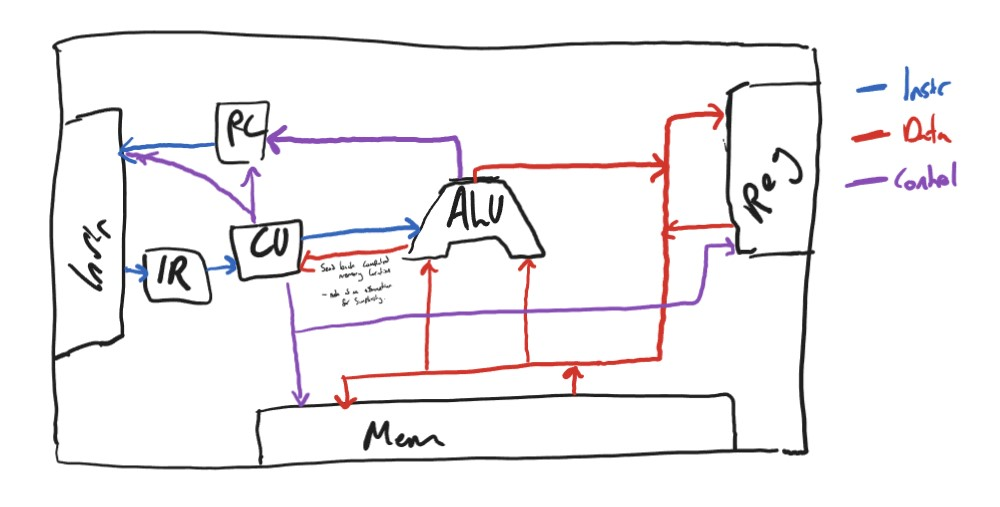
\includegraphics[width=\linewidth]{dissertation/DATA/animation_layout.jpg}
    \caption{Original animation area design}
    \label{fig:early_animation_design}
\end{figure}

\begin{figure}[H]
    \centering
    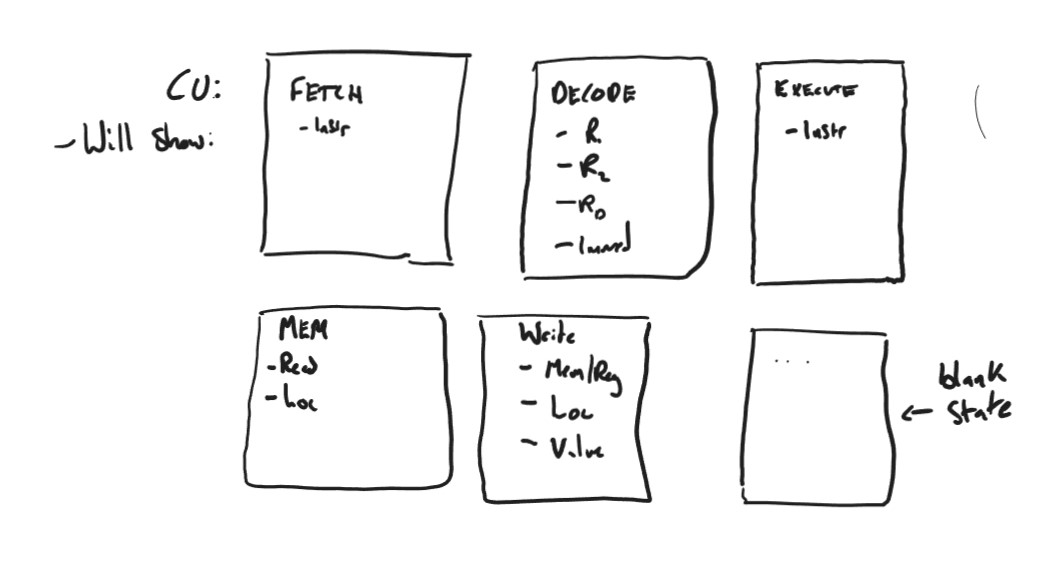
\includegraphics[width=\linewidth]{dissertation/DATA/control_unit.jpg}
    \caption{Original Control Unit design}
    \label{fig:early_cu_design}
\end{figure}

Figure \ref{fig:early_animation_design} displays the concept of the animation area, with components being connected by coloured wires. With blue, red and black representing the transfer of Instructions, Data and Control signals respectively. Larger boxes allocated to side elements, correspond to the respective Register, Memory and Code \ac{UI} elements on the wider interface.

The \ac{CU} in Figure \ref{fig:early_animation_design} is displayed as a simple box. It is intended that this will display more data to convey what the emulator is doing. For example it may display the currently executing stage and some information associated with the stage. Examples of this more detailed design can be seen in Figure \ref{fig:early_cu_design}.

These base designs allowed us to then revise and redesign to improve aspects and usability. During revisions we decided to consider Nielsen's Usability Heuristics \cite{nielsen_2020_10} as covered in section \ref{sec:nielson}. Within this, our design failed 2 principles, being 1 and 8 relating to visibility of system status and aesthetic and minimalist design respectively.

The design failed these due to our choice to redesign to include colour within our interface to help differentiate the animation components. This lead to the use of colours such as red and green which colourblind users are unable to differentiate between, instead appearing as a murky brown. To prevent this issue whilst also maintaining this newer design we switched to using grayscale. This eliminated the issue whilst still providing a way for colourblind users to easily differentiate between processor components and thus making the visibility of the system better available to all.

A further design issue was a choice of background colour. With the original change using a gray background instead of white, going with a dark-ish gray. However, this produced a low contrast ratio between the background and other element, which may prove hard for visually impaired users to see as-well as increasing eye strain. 

The Web Accessibility Initiative \cite{webaccessibilityinitiativew3_2022_understanding} denotes a minimum contrast ration of 4.5:1, which our original design of gray on gray violates. Upon further redesigning the choice to switch the dark gray for a much lighter gray was made. This decision greatly increased the contrast ratio to an acceptable level.

An overview of the above changes and a few extra to improve usability are listed below:
\begin{enumerate}
    \item Lightening of the background to increase the contrast ration to an acceptable level,
    \item Convert the red, green and blue boxes to grayscale to alleviate the issue for colourblind users,
    \item Switched gray boxes to purple to increase contrast against the background.
\end{enumerate}

With all these consideration taken into account the final design was complete, with a physical mock up generated as seen in Figure \ref{fig:final_implemented_design}. (Please note this image has been taken from our implemented design, which has no major changes from the designed version).

\begin{figure}[H]
    \centering
    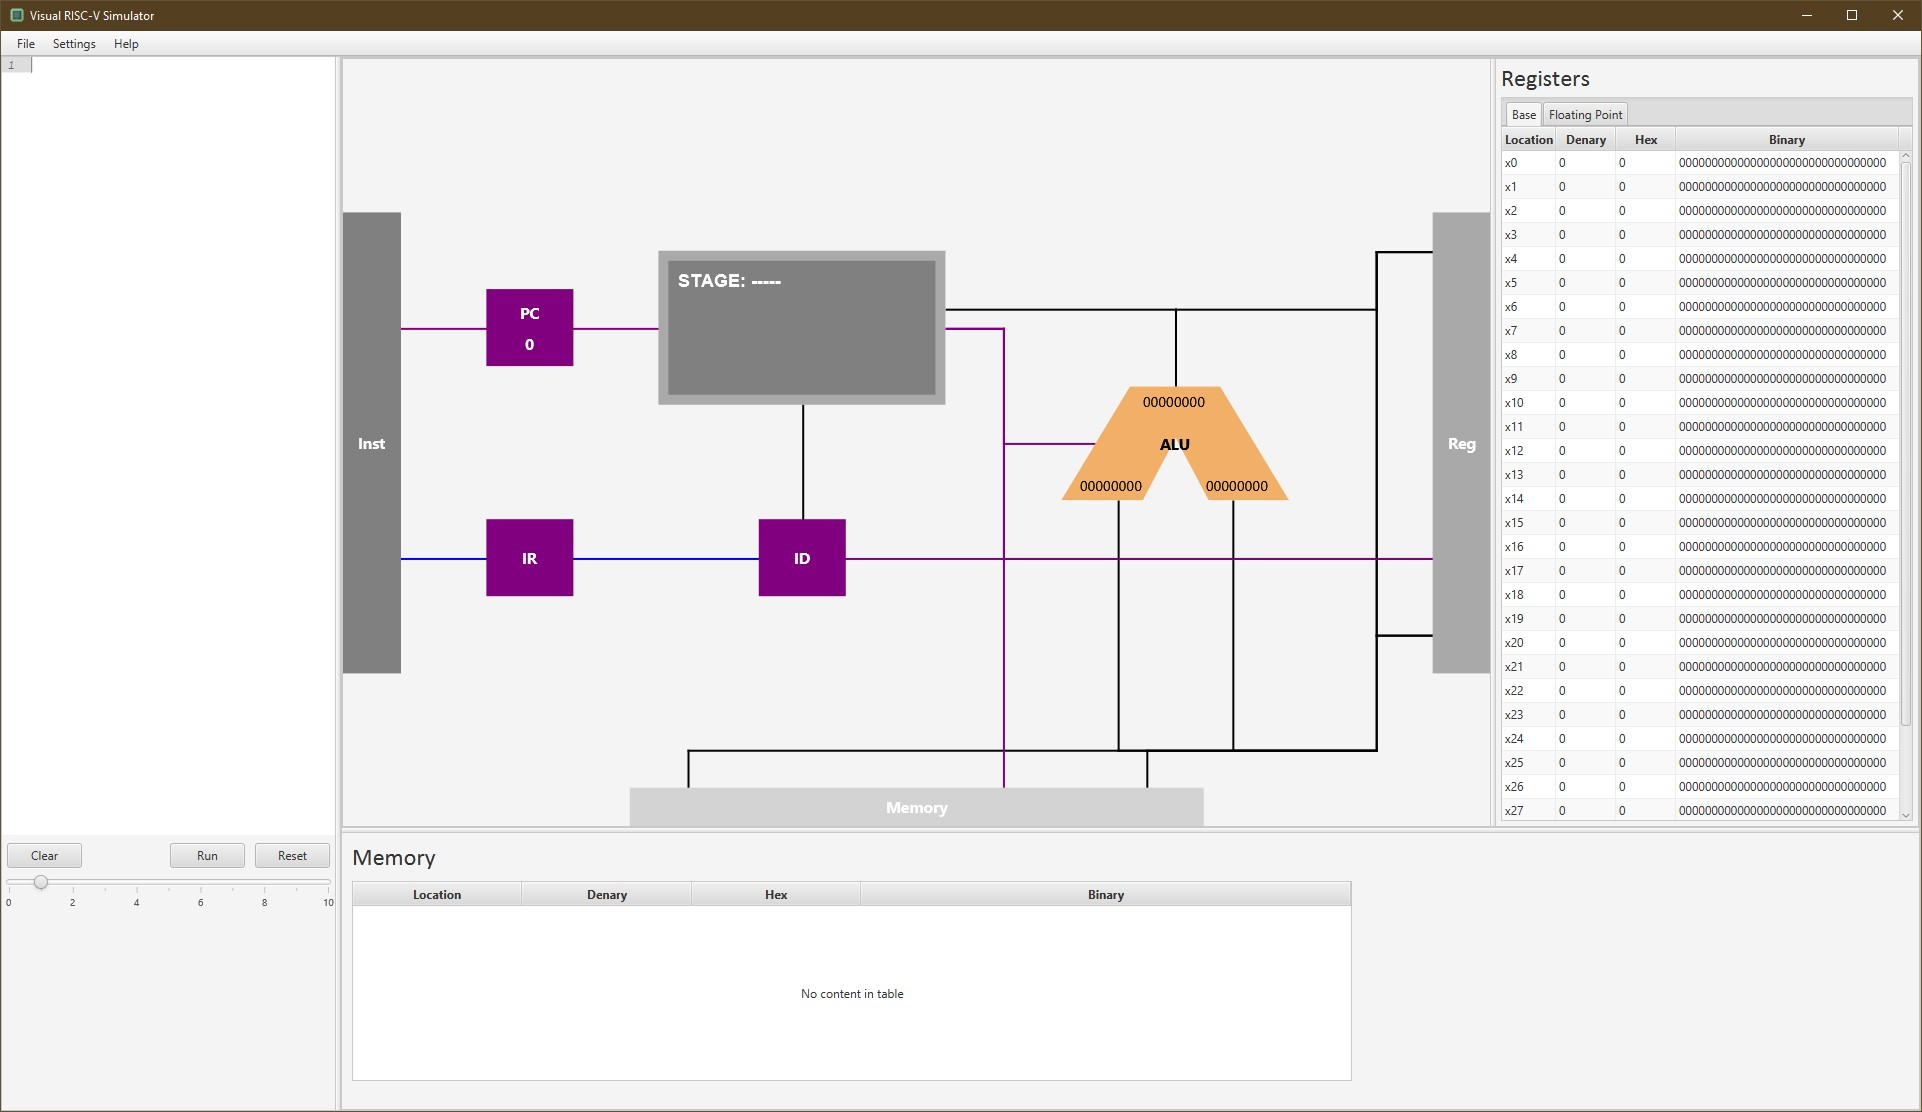
\includegraphics[width=0.9\linewidth]{dissertation/DATA/final_design.jpg}
    \caption{Final full UI design}
    \label{fig:final_implemented_design}
\end{figure}

This final design allows us to follow Nielsen's 10 principles \cite{nielsen_2020_10}, with an intuitive and minimalist design, retaining only what's required on screen. Further following principle 4 by keeping our layout and design consistent across the entire application.

\section{Module System}\label{sec:module}
The applications module system is designed to be convenient and easy to use. As mentioned at the start of the design section, modules are implementations of RISC-V extensions and were a later addition that was designed around the emulator. Thankfully, due to our simple emulator design the Module system could be easily designed, providing the ability to directly add new instructions and features into the system.

\begin{figure}[H]
    \centering
    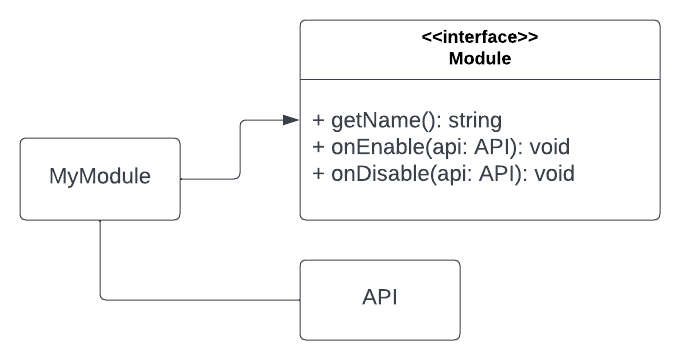
\includegraphics[width=0.9\linewidth]{dissertation/DATA/module uml.png}
    \caption{Module System UML Diagram}
    \label{fig:module_uml}
\end{figure}

Modules are designed to implement a base module interface as seen in Figure \ref{fig:module_uml}, with the system designed to be able to independently find and load modules and then enable and disable them as required. Modules are designed to be quick to create which allows for more focus on the implementation of custom logic, with enable and disable methods provided to instantiate and cleanup module features as required.

Modules are also designed to be provided with access to an API as seen in Figure \ref{fig:module_uml}. This API is designed to be simple, allowing modules to access the the emulator, without directly exposing the core system.

The overarching system managing individual modules was also designed to be simple, with an option to quickly enable and disable modules, as well as a simple interface to load and remove modules.

Figure \ref{fig:module_popup} shows an example of the module popup, which will allow users to manage their modules, as well as enable and disable them.

\begin{figure}[H]
    \centering
    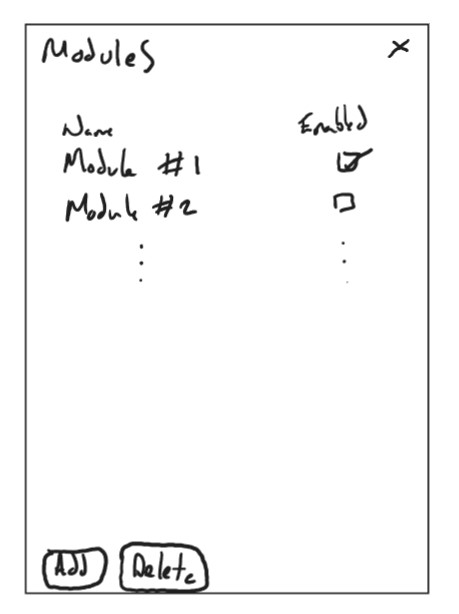
\includegraphics[width=0.7\linewidth]{dissertation/DATA/module design.jpg}
    \caption{Module popup design}
    \label{fig:module_popup}
\end{figure}


